\documentclass{article}
\usepackage{syntax}
\usepackage{tikz}
\usetikzlibrary{automata, positioning}

\begin{document}
    %Notizen
    folgende Begriffe sollen definiert werden:

    Visual Programming Language

    Grammatik

    Domain Specific Language

    Schleifen

    Flowchart

    (Fixpunktberechnung)
    \newpage
    \tableofcontents
    %Einleitung
    \newpage
    \section{Einleitung}
    %Haupteil
    \newpage
    \section{Aufbau der domainspezifischen Sprache}
    Im nachfolgenden Kapitel möchte ich die zugrundeliegende Grammatik beschreiben. Am Anfang möchte ich auf die Notation eingehen.\\\\
    Die zugrundeliegende Grammatik basiert auf der Backus-Naur-Form (BNF) Notation. Der Aufbau einer BNF wird anhand der Grammatik~\ref{BNF} erklärt
    <symbol> sind nichtterminale
    ::= bedeutet dass symbol durch _expression_ ersetzt wird
    _expression_ ist eine sequenze von nichterminalen und terminale
    Kleene-Stern * wiederholung
    Alternation \textbar  oder
    Sequenz erlaubt auch Klammern um die Reihenfolge der Regel zu definieren
    Softwareprüfung lääst sich visuall von zwei seiten betrachen. 
    \begin{grammar}
        <symbol> ::= _expression_
    \end{grammar}
    \textbf{Grammatik TODO} Backus-Naur-Form\\\\\\
    \label{BNF}
    Grammatik lässt sich in 3 Ebenenunterteilen Prüfungslogik, Datenverarbeitung und Typsystem
    Prüfungslogik führt Entscheidung im Prüfungsablauf aus und bestimmt die Reihenfolge der Aktionen. außerdem datenerfassung
    Datenverarbeitung ist für die Datentranformation auswertung zustädnig. Also Funktionen, welche keine Nebeneffekte besitzen, weil sie unabhängig von der restoichen Softwareprüfung stattfinden.
    Typsystem ermöglicht die statische analyse der ausführbarkeit
    Softwareprüfung lääst sich visuall von zwei seiten betrachen. 
    Einmal als Datenflussgraphen, indem Teil-Funktionen als Blöcke dargestellt werden und Funktionsparamter/Ergebnisse als Ports.
    Einmal als Aktivitätsdiagramm, in dem nur Startzustand, Endzustände, Aktions- und Entscheidungsblöcke dargeste
    \subsection{Prüfungslogik}
    Das Aktivitätsmodell  $<ActivityModel>$ besteht aus einer Reihe von Aktivitäten $<Activity>$.
    Aktivitäten können dabei entweder eine Startmarkierung, eine Aktivitätsaktion, einem Vergleich oder visualles Label sein.
    Die Startmarkierung muss pro Prüfungslogik genau einmal vorkommen.
    Ein vergleich kann dabei entweder eine Binärentscheidung oder eine Validierungsentscheidung sein.   
    Die Validierungsentscheidung nimmt als Eingabe einen Wert und überprüft ob diese Werte vorhanden sind.
    Die Binärentscheidung nimmt als Parameter zweite Werte, einen Vergleichoperatur und eine referenz zu einer Funtkion. Dabei werden beide Werte als Eingabe für die referenzierte Funktion verwendet.
    Als Vergleichoperatoren stehen $=$ und $\neq$ sowie Relationale Operatoren zur verfügung.
    Eine Aktivitätaktion <ActivityAction> kann dabei einer der folgenden Aktionen ausführen:
    Bevor das Ergbeniss aus der vorherigen Aktionsaktivität verwendet wird, kann eine Transformation auf dieses Ergebniss angewendet werden.
    \begin{itemize}
        \item Senden von Hauptuntersuchungs-Adatper-Anfragen (A1)
        \item Lesen einer JSON Datei (A2)
        \item Ausführung einer Datenverarbeitung (A3)
    \end{itemize}
    A1 nimmt als Parameter den Namen der auszuführenden Anfrage, eine Beschreibung für den debugger, eine Liste von anzusprechnenden System im Fahrzeig und die maximale Zeitdrauer einer Anfrage.
    A2 nimmt als Eingabe den Typ der zu ladenenden Datei und die dazugehörige URI.
    A3\\
    \begin{grammar}
        <ActivityModel> ::= <Activity>* <ActivityConnection>

        <Activity> ::= <ActivityStart>
        | <ActivityAction>
        | <ActivityCondition>
        | <ActivityDisplay>

        <ActivityStart> ::= $\epsilon$

        <ActivityAction> ::= <ActivityFlowCall>
        | <ActivityPitaBuildInforRequest>
        | <ActivityLoadExternalData>

        <ActivityFlowCall> ::= ref(FlowTemplate) <ActivityPortValue>* <TemplateParameterValue>* <ValueTransformation>*

        <ActivityPitaBuildInforRequest> ::= <string abdFilename> <string requestAlias> <string expectedSystems>* <number timeout>

        <ActivityLoadExternalData> ::= <Type dataType> <string dataSource>

        <ActivityPortValue> ::= <FlowPortValue>
        | <ActivityPortRefernce>

        <FlowPortValue> ::= <string>
        | <number>
        | <bool>
        | <date>
        | <FlowPortValue>*

        <ActivityPortRefernce> ::= ref(ActivityAction) (ValueTransformation)*

        <ValueTransformation> ::= <string objectReference>
        | <number listIndex>

        <ActivityCondition> ::= <ActivityBinaryCondition>
        | <ActivityValidityCondition>

        <ActivityBinaryCondition> ::= ref(FlowTemplate) <ActivityBinaryConditionOperator> <ActivityPortValue left> <ActivityPortValue right>

        <ActivityValidityCondition> ::= <ActivityPortValue>*

        <ActivityBinaryCondition> ::= '='
        | '$\neq$' 
        | '\textless' 
        | '$\leq$' 
        | '\textgreater' 
        | '$\geq$'

        <ActivityDisplay> ::= <ActivityDisplayField>*

        <ActivityDisplayField> ::= <string label> <string color> ref(ActivityAction)
    \end{grammar}
    \textbf{Grammatik TODO} Aktivitätsmodell
    \newpage
    \subsection{Datenverarbeitungs}
    Eingabe <FlowInputPort> und Ausgabe $<FlowOutputPort>$
    Funktionen höherer Ordnung $<FlowLamda>$
    Eine Funktion höher Ordnung besteht aus zustzälciehn Eingabe- und Ausgabeports
    Eingabe- und Ausgabeports nehmen als Parameter einen Namen des Ports, den Typ und ob Fehlererlaub ist.

    Ein Funktions Template $<FlowTemplate>$ besteht aus einer Funktion $Flow$ und belieg vielen Parametern $<TemplateParameter>$
    Die Parameter generieren Port- und Lambda-Defintion
    Funktionen welche vom Autorensystem $<LibraryFlow>$ und selbst definierte Funktionen $<FlowModel>$

    Ein Flow-Modell ist ein DAG bei dem mehrere Funktionen mitienander verbunden werden. Einzelne Funktionen werden Nodes $<FlowNode>$ genannt.
    Das Flow-Modell wird durch eine $<FlowInstance>$, Reihe von Funktionen und Verbidnugen definiert.
    Die Funktion kann dabei eine Eingabe <$FlowNodeInput>$, eine Ausgabe $<FlowNodeOutput>$, einer Lambda Referenz $<FlowNodeLambda>$ oder eine Funtkions Referenz $FlowNodeFlowCall$
    Konstante Werte $FlowPortValue$
    \begin{grammar}
        <FlowInstance> ::= <FlowOutputPort lambdaArguments>* <FlowInputPort lambdaArguments>* <FlowLambda>*
        
        <FlowLambda> ::= <FlowOutputPort lambdaArguments>* <FlowInputPort lambdaArguments>*

        <FlowInputPort> ::= <string name> <Type> <bool acceptsError>

        <FlowOutputPort> ::= <string name> <Type> <bool producesError>
    \end{grammar}
    \textbf{Grammatik TODO} Flow-Instanz
    \begin{grammar}
        <FlowTemplate> ::= <Flow> <TemplateParameter>*

        <Flow> ::= <LibraryFlow> | <FlowModel>
        
        <LibraryFlow> ::= $\epsilon$

        <TemplateParameter> ::= 'String' | 'Number' | 'Bool' | <TemplateParameterList>
        
        <TemplateParameterList> ::= <TemplateParameter>
    \end{grammar}
    \textbf{Grammatik TODO} Flow-Template
    \begin{grammar}
        <FlowModel> ::= <FlowInstance> <FlowNode>* <FlowConnection>*

        <FlowNode> ::= <FlowNodeOutput> | <FlowNodeInput> | <FlowNodeLambda> | <FlowNodeFlowCall>
       
        <FlowNodeOutput> ::= ref(FlowOutputPort) <FlowPortValue>

        <FlowNodeLambda> ::= ref(FlowLambda) <FlowPortValue>*

        <FlowNodeFlowCall> ::= ref(FlowTemplate) <FlowPortValue>* <TemplateParameterValue>*
    
        <FlowConnection> ::= ref(FlowOutputPort source) ref (FlowOutputPort target)
    
        <FlowConnection> ::= ref(FlowOutputPort source) ref (FlowOutputPort target)
    
        <TemplateParameterValue> ::= <string> | <number> | <bool> | <TemplateParameterValueList>
    
        <TemplateParameterValueList> ::= <TemplateParameterValue>*
    \end{grammar}
    \textbf{Grammatik TODO} Flow-Modell
    \newpage
    \subsection{Typsystem}
    unterstüzt die gleichen Primitiv-Typen wie JSON-Format String, Number und Bool zusätzlich Date und PtiaResponse. Außerdem werden auch gernerische Typen unterstüztz, weil nicht immer von vorneherein der Typ bekannt ist.
    Date ist eine Datumsangabe
    PtiaResponse ist eine Antwort einer Hauptuntersuchungs-Anfrage
    Diese Typen lassen sich an optionalen, Listen oder Objekt-Typen kapseln\\
    \begin{grammar}
        <Type> ::= <TypePrimtive> | <TypeOptional> | <TypeList> | <TypeObject>

        <TypePrimtive> ::= 'String' | 'Number' | 'Bool' | 'Data' | 'PtiaResponse'
        
        <TypeOptional> ::= <Type> '?'
        
        <TypeList> ::= <Type> '[]'
        
        <TypeObject> ::= '\{' (<string key> ':' <Type>)* '\}'

        <TypeGeneric> ::= '\$' <string genericName>

        <TypeReference> ::= ref(Type)
    \end{grammar}
    \textbf{Grammatik TODO} Typ-Defintion mit generischen und Referenz-Typen
    \newpage
    \section{Implementierung}
    Bei der Implementierung muss nicht nur auf des Design des Schleifenkonstrukt geachtet werden, sondern auch auf neue Sachen, welche durch die Implementierung entstanden sind.
    Bei den Schleifendurchläufen wird nicht auf die Ergebnisse des letzten Durchlaufs zugegriffen werden, sondern der Schleifenkörper soll die Entscheidungen auf Grundlage des aktuellen Sensorwertes treffen.
    Das auslesen des aktuellen Sensorwerts ist bereits möglich.
    Aktuell unterstützt die zugrundeliegenede Implementierung noch keine Variablen. Um das zu ändern muss die Grammatik bearbeitet werden-
    \subsection{1. Lösungsansatz}
    %Ausformulierte Notizen. 
    Der Benutzer gibt von vorneherein eine Zahl a an, welche die maximale Anzahl von Schleifendurchläufe beschränkt. Für die Zahl muss dafür folgendes gelten TODO.
    Die Idee des Ansatzes ist es, den Schleifenköper nicht Iterativ oder Rekursiv ausführen, sondern a-mal auszurollen.
    Dafür wird der Schleifenköper und die nachfolgenden Anweisungen a-mal kopiert. Die Schleife wird dadurch nicht dynmasisch ausgeführt, sondern statisch in den Code implementiert. Dadurch entstehen $a+1$ Graphen. Jeder dieser Graphen repräsentiert einen ursprüngliche Iteration. Dabei werden die einzelnen Graphen mit ihren direkten Nachbaran verbunden. 
    Da die aktuell zugrunde liegende Implementierung determenistisch ist und aktuell nur auf die gleiche Eingabe zugegriffen werden kann, muss ein Mechanismus implementiert werden, welcher den aktuellen Sensorwert ausliest und diesen an die nachfolgenden Anweisungen weitergibt. Dieser Vorgang muss für jede neu eingefügte Verbindung wiederolt werden.
    Dieser Ansatz wird auch von Ye et al. im Konferenz-Paper "Loop Unrolling Based on SLP and Register Pressure Awareness" beschrieben.\\
    \resizebox*{!}{10cm}{
    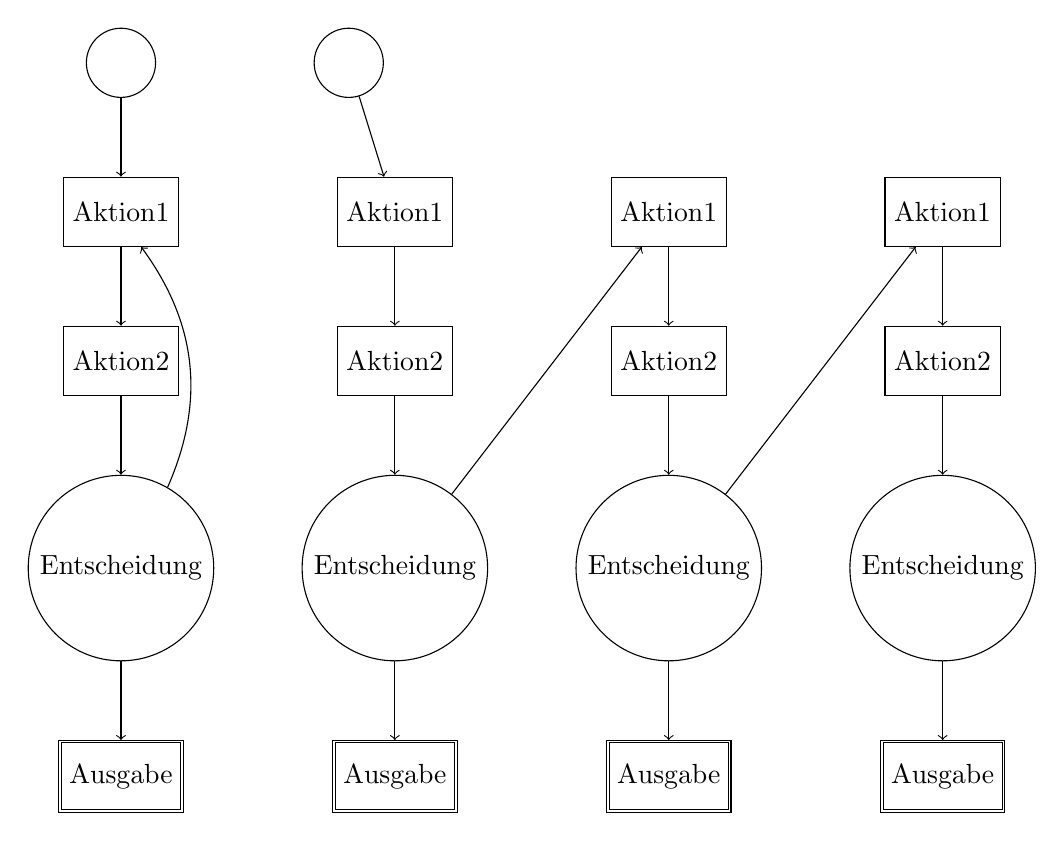
\begin{tikzpicture}[]
        %Graph links
        \node[state, initial text=""](q0){};
        \node[state, rectangle, below = 1cm of q0](q1){Aktion1};
        \node[state, rectangle, below = 1cm of q1](q2){Aktion2};
        \node[state, below = 1cm of q2](q3){Entscheidung};
        \node[state, accepting, rectangle, below = 1cm of q3](q4){Ausgabe};

        \draw(q0) edge[->] (q1);
        \draw(q1) edge[->] (q2);
        \draw(q2) edge[->] (q3);
        \draw(q3) edge[->, bend right] (q1);
        \draw(q3) edge[->] (q4);

        %Graph rechts
        \node[state, initial text="", right = 2cm of q0](q5){};
        \node[state, rectangle, right = 2cm of q1](q6){Aktion1};
        \node[state, rectangle, right = 2cm of q2](q7){Aktion2};
        \node[state, below = 1cm of q7](q8){Entscheidung};
        \node[state, rectangle, accepting, below = 1cm of q8](q9){Ausgabe};

        \node[state, rectangle, right = 2cm of q6](q10){Aktion1};
        \node[state, rectangle, right = 2cm of q7](q11){Aktion2};
        \node[state, below = 1cm of q11](q12){Entscheidung};
        \node[state, rectangle, accepting, below = 1cm of q12](q13){Ausgabe};

        \node[state, rectangle, right = 2cm of q10](q14){Aktion1};
        \node[state, rectangle, right = 2cm of q11](q15){Aktion2};
        \node[state, below = 1cm of q15](q16){Entscheidung};
        \node[state, rectangle, accepting, below = 1cm of q16](q17){Ausgabe};

        \draw(q5) edge[->] (q6);
        \draw(q6) edge[->] (q7);
        \draw(q7) edge[->] (q8);
        \draw(q8) edge[->] (q9);
        \draw(q8) edge[->] (q10);
        
        \draw(q10) edge[->] (q11);
        \draw(q11) edge[->] (q12);
        \draw(q12) edge[->] (q13);
        \draw(q12) edge[->] (q14);

        \draw(q14) edge[->] (q15);
        \draw(q15) edge[->] (q16);
        \draw(q16) edge[->] (q17);


    \end{tikzpicture}
    }
    \\\textbf{Abbildung TODO} Algorithmus Schleifenentfaltung\\
    \\Auf die Vor- und Nachteile der Implementierung wird im Kapitel~\ref{Evaluation} eingegangen.
    \subsection{2. Lösungsansatz}
    Wie auch schon beim 1. Lösungsansatz gibt der Benutzer von vorneherein eine Zahl a an, welche die Anzahl an Schleifendurchläufen beschrnänkt. Für die Zahl a gelten die gleichen Bedingungen wie im 1. Lösungsansatz beschrieben. 
    Zusätzlich wird noch eine Zahl TODO benötigt, welche auch der Benutzer angeben muss. TODO soll dabei die Funktionen eines Grenzwertes übernehmen.
    Bei diesem Ansatz werden mehrere Mittelwerte gebildet und geschaut, wie sich der neu ausgelesene Sensorwert sich im Verhältnis zu den Mittelwerten verhält. Es wird die Differenz zwischen Mittelwert und aktuellen Sensorwert gebildert. Anschließend wird geschaut auf die Differenz größer als TODO ist.
    Die Mittelwerte bilden wir einmal über alle bisherigen Sensorwerte und einmal über die letzten b Sensorwerte. Dadurch haben wir die Mittelwerte für einen kurzen und längeren zeitraum.
    Sollte das der Fall sein, wissen wir das die Sensorwerte sich noch nicht stabilisiert haben und wir können den Vorgang wiederholen. Da wir nicht bereits nachdem ersten stabilisierten Wert aufhören wollen, sondern erst wenn der Wert über einen längeren Zeitraum stabil ist, führen wir folgenden n-Chance-Mechanismus ein:
    \begin{itemize}
        \item Sollte der Grenzwert unterschritten werden, wird der Counter um 1 erhöht.
        \item Sollte der Grenzwert überschritten werden, wird der Counter wieder auf 0 gesetzt.
        \item Sollte der Counter irgendwann n erreichen, wissen wir das sich die Werte stabilisiert haben und wir davon ausgehen können dass das zu erwartende Ergebniss nicht mehr rauskommt.
    \end{itemize}
    %Schluss
    \newpage
    \section{Evaluation}
    \label{Evaluation}
    \subsection{}
    \subsubsection{1. Lösungsansatz}
    +einfach zu implementieren, da wir kein schleifenkonstrukt mehr benötigen.
    +keine Endlosschleife, weil es keine Schleifen gibt
    +keine Zyklen, weil der Ablauf linear ist
    +weniger Sprünge, weil keine for oder while Bedingungen vorhanden sind
    +möglicher Performance gewinn, weil Schleifen-Overhead entfällt
    -größerer Codeumfang, da der eigentliche schleifenkörper a-mal im code implemtniert werden muss 
    -höherer verbraucht an ressourcen zB Speicher mehr code = mehr speicher
    -möglicherweise ineffizient, wenn der faktor zu groß gewählt wird
    -schlechtere Lesbarkeit
    -wenn bereits nach 3 durchlaufen feststeht, dass das gewünschte ergbeniss nicht mehr erreicht werden kann werden trotzdem die restlichen schritte ausgeführt
\end{document}    